
\chapter{EMC Simulation}Nuclei are systems of nucleons that interact strongly. The characteristic scale for the nucleons momentum is approximately the Fermi momentum, $k_F \approx 200-270 MeV/c$ \cite{gomez}. However because of the strongly repulsive nature of the nucleon-nucleon interaction at short distances prevents two nucleons from laying in close proximately to each other. This strong interaction demands the presence of high-momentum components in the nuclear ground state wave function. A simulation was designed to phenomenologically study the effect of these high-momentum components on the nuclear EMC effect. This program was designed in two phases. The first phase used simple elastic scattering and a single value for the targets momentum to investigate overall effect of different target momentum on the yield in bins of $x_B$. The second phase of the simulation was created to lay out the effect of using different momentum distributions on the yield for the EMC effect region of $x_B$, 0.3 to 0.7.
\section{Investigation} This simulation phenomenologically investigates the effect of a moving target on the EMC effect by scattering a beam of electrons off of a moving proton. The target protons are comprised of a directional vector of 0$^\circ$ to 360$^\circ$ in respect to the incoming electron beam and a momentum between 0 and 1 GeV/c. Figure \ref{example} contains a possible event for the simulation. The electron approaches with 2.5 GeV of energy and collides with a proton moving with a momentum of 0.5 GeV/c with an angle of 45$^\circ$ in respect to the electron trajectory. 
\begin{figure}[t]
\centering
\caption{Example of the electron beam(red) with a energy of 2.5 GeV and the proton(blue) with angle of 45$^\circ$ in respect to the electron and with a momentum of 0.5 GeV/c.}
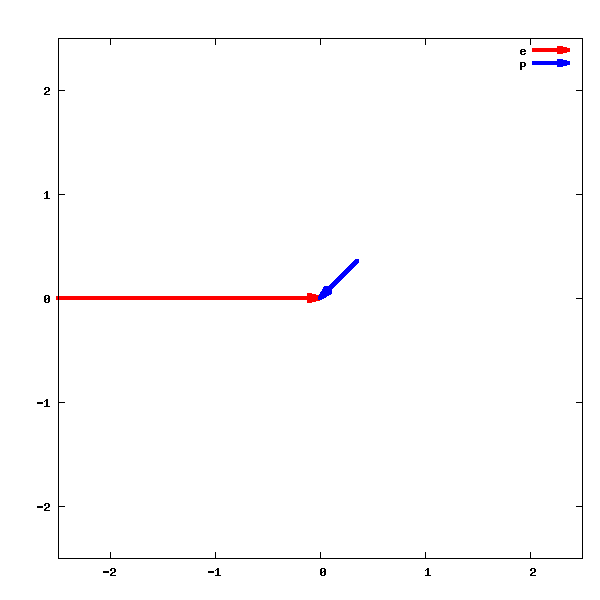
\includegraphics[width=8cm]{Initial.png}
\label{example}
\end{figure}

Using conservation of momentum and conservation of energy in elastic collisions, this simulation calculates the final state of the electron and proton after the scattering event by randomly selecting a scattered direction for the electron. The vector representation of the scattered products are shown in figure \ref{boom}. In order to make these calculations systematic and to study cross sections models the simulation transform each event into the rest frame of the target before scattering. 

\section{Transformation}
The Simulation completes a set of Lorentz invariant  rotations and boost for each event to transform the lab frame of the electron and proton collision into the rest frame of the proton. First the simulation takes the initial proton and electron vectors and rotates them to align the proton vector to the horizontal axis, shown in figure \ref{LAM}.This rotation uses the angle between the proton and the electron defined as $\lambda$. This allows for a straight forward calculations for the Lorentz factors $\beta$ and $\gamma $ and to boost into the rest frame of the target proton, figure \ref{boost}. Once in the boosted frame, the angle between the electron and the horizontal axis is defined as $\delta$.  Right before the simulation starts to calculate the scattered products, it completes one more rotation to align the electron vector with the horizontal axis, figure \ref{delta}, to make the scattering calculation systematic and unconditional. 

\begin{figure}[t]
  \centering
  
  \subfloat[Initial Vectors]{
  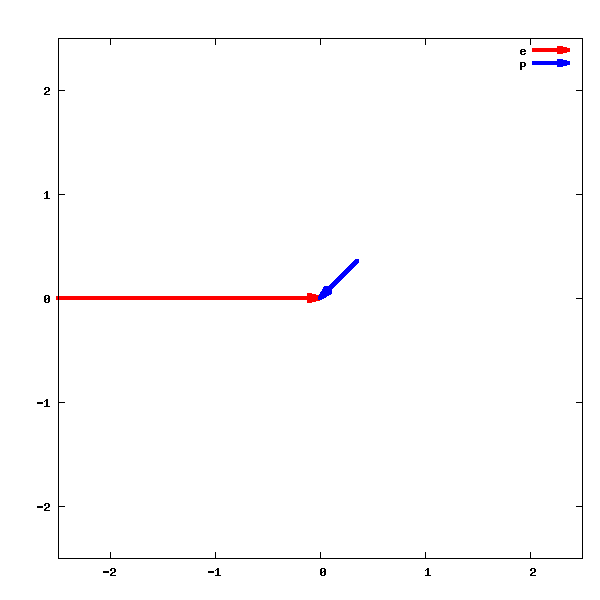
\includegraphics[width=6.5cm]{Initial.png}
  \label{IV}}
  \quad
  \centering
  \subfloat[Rotated by Lambda]{
  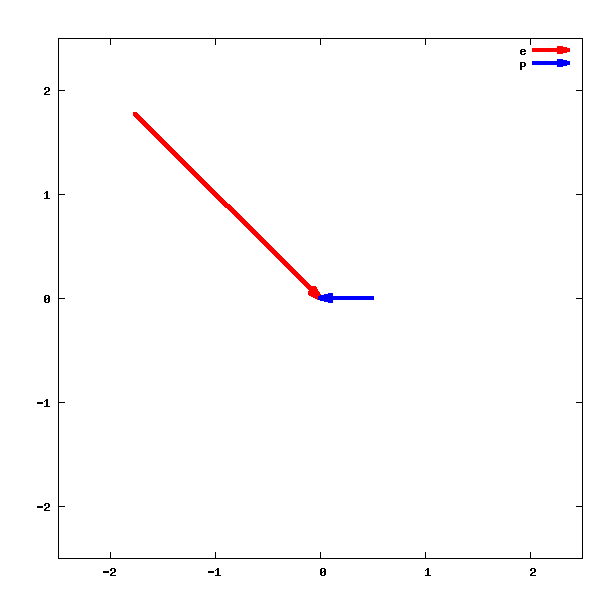
\includegraphics[width=6.5cm]{RotatedbyLam.png}
  \label{LAM}}
  \vspace{-2cm}
  \centering
  \subfloat[Boosted]{
  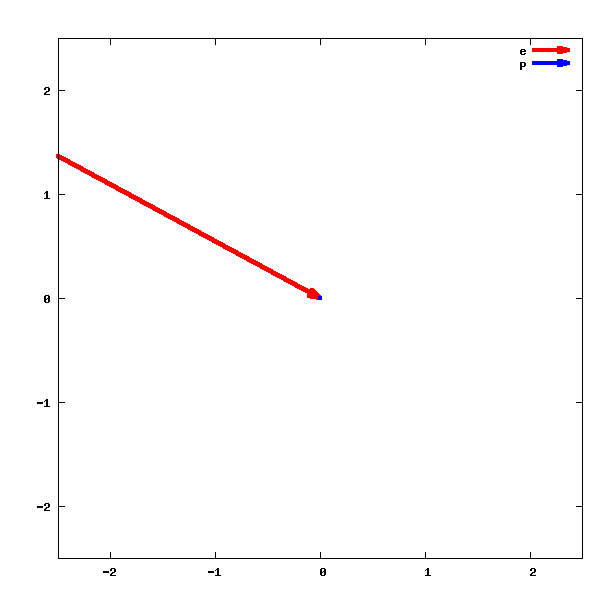
\includegraphics[width=6.5cm]{boosted.png}
  \label{boost}}
  \quad
  \centering
  \subfloat[Before being scattered]{
  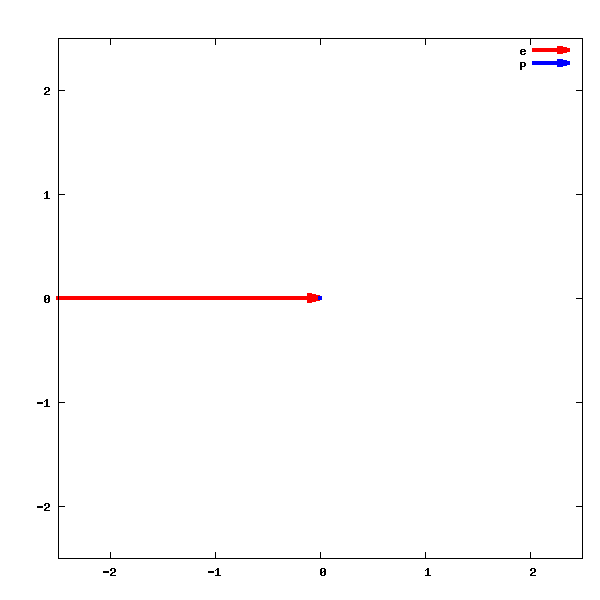
\includegraphics[width=6.5cm]{beforescattering.png}
  \label{delta}}
  
  \caption{Vector representations of the momentum for the incoming electron(red) and  target proton(blue) with units of GeV for each phase of their transformations before scattering.}
  \label{transform}
  \end{figure}
  
  In order to gain a more complete understanding of the scattering products, the program completes a set of transformations to move from the rest frame of the target proton to the beginning lab frame. After the simulation calculates the scattered products it begins to transform back by beginning with a rotation by the angle $\delta$, figure \ref{delta2}. Followed by the inverse of the previously used Lorentz boost. The last transformation, a rotation by $\lambda$, transforms the frame back into the lab frame. A proton vector and electron vector in the lab frame are the final products of the simulation. An image of the electron and proton vectors for each transformation can be found in figure \ref{transform2}. These vectors allow for calculation of kinematic variables such as Bjoken $x$ and the four-momentum transfer ($Q^2$).  This simulation will complete these steps for many electron and proton combinations.
  \begin{figure}[h]
    \centering
    \subfloat[After scattering]{
    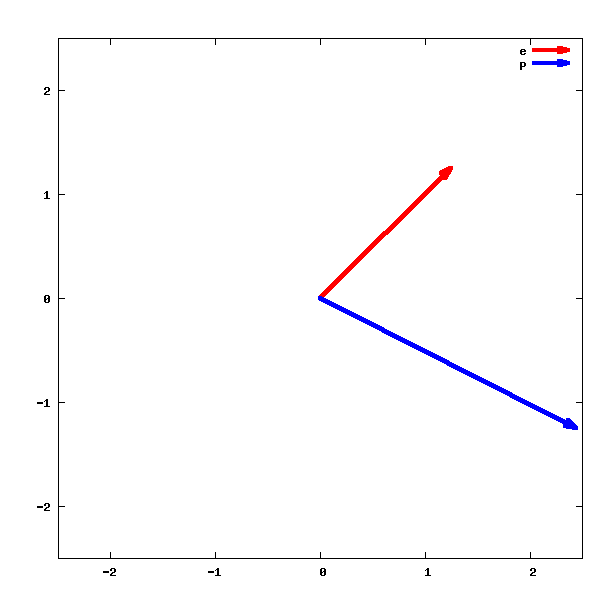
\includegraphics[width=7.0cm]{afterscatter.png}
    \label{boom}}
    \quad
    \centering
    \subfloat[Rotate back by $\delta$]{
    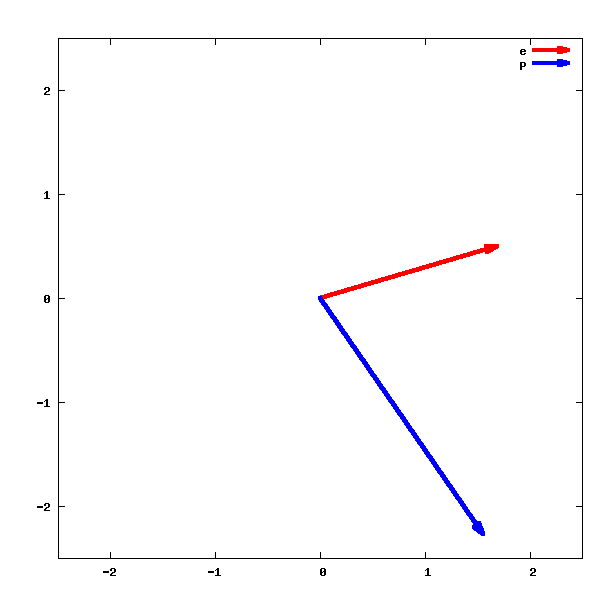
\includegraphics[width=7.0cm]{Rotatedbydelta.png}
    \label{delta2}}
    \vspace{-1cm}
    \centering
    \subfloat[Boosted]{
    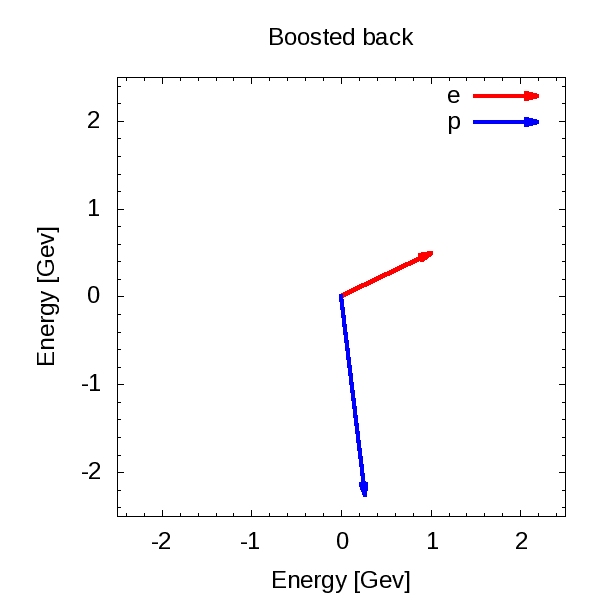
\includegraphics[width=7.0cm]{boostedback.png}
    \label{boost2}}
    \quad
    \centering
    \subfloat[Final vectors]{
   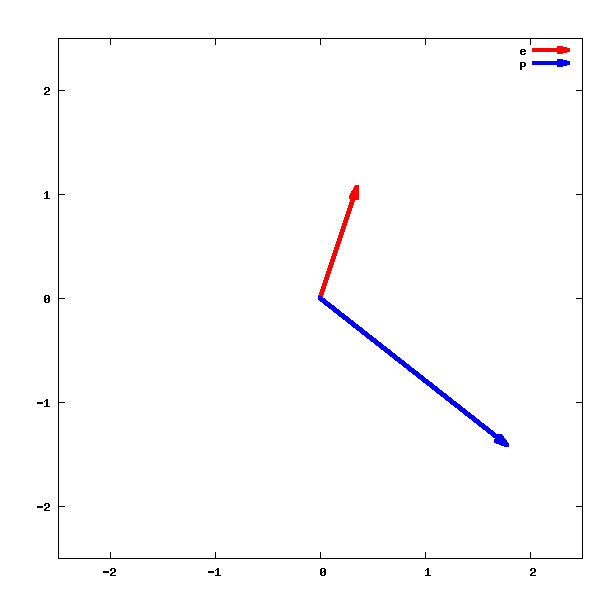
\includegraphics[width=7.0cm]{final.png}
    \label{Final}}
    
    \caption{Vector representations of the momentum for the incoming electron(red) and  target proton(blue) with units of GeV for each phase of their transformations after scattering).}
    \label{transform2}
    \end{figure}


\section{Results}
This electron scattering simulation produced results for two stages. The firsts stage used a fix proton momentum for each run to compare the yield in bins of $x_B$. Figure \ref{ES_res} shows the results for three different runs, each having a unique fixed proton momentum. The red histogram represents a run with a proton momentum of 0 Gev/c. The result is an elastic peak at $x_B$ of one. The blue histogram contains the results having a fixed proton momentum of 0.25 GeV/c. Increasing the initial momentum of the proton spreads the events into two peaks. The scattering interactions that form the peak above 1 $x_B$ are produced by events were the proton's initial directional vector are orientated towards the electron.  The events that produce an $x_B$ below 1 have a proton direction pointing away from the electron initially. Doubling the proton's initial momentum from 0.25 GeV to 0.50 GeV causes these peaks two spread out furtherer in $x_B$.  


\begin{figure}[h]
\centering
\caption{Simulation results for fixed momentum protons. Three runs with unique proton momentum. }
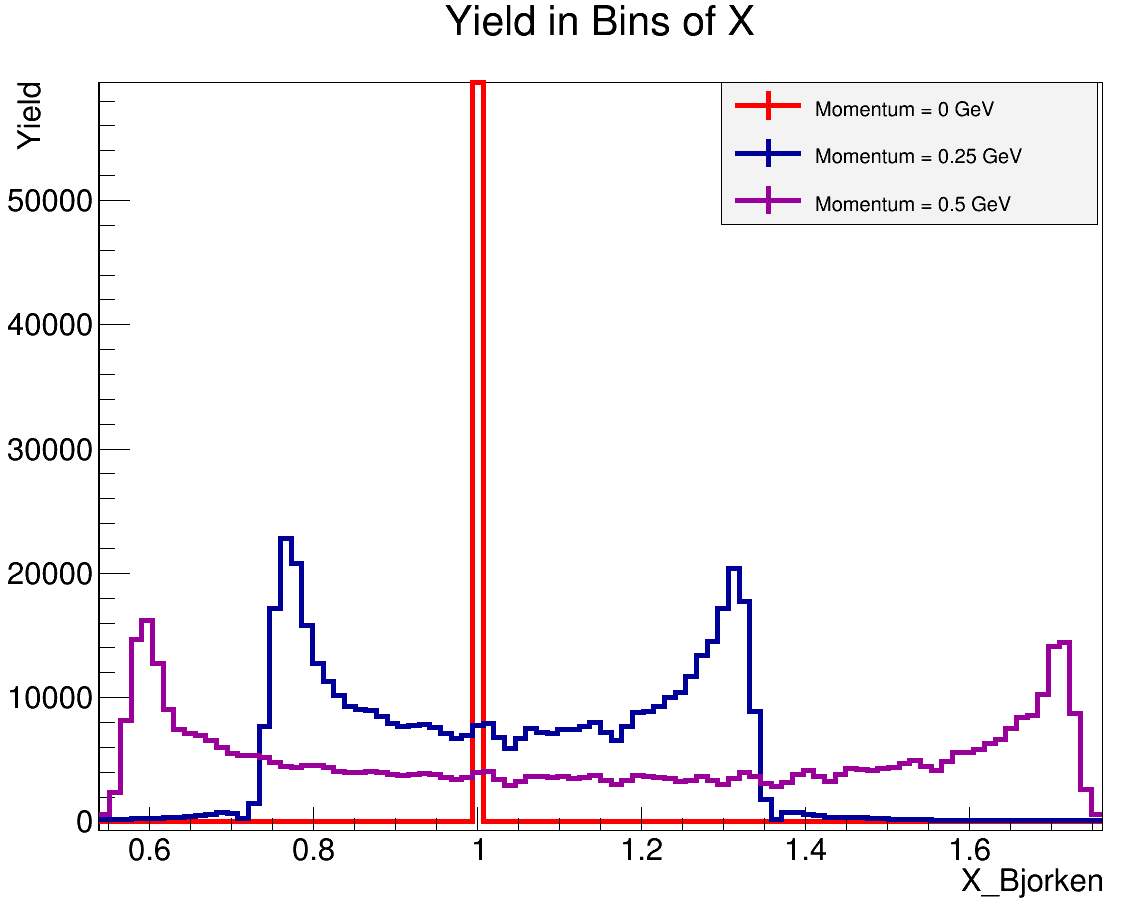
\includegraphics[width=15cm]{Es_results.png}
\label{ES_res}
\end{figure}

